\chapter{Experimentos}
Siguiendo la estructura planteada a lo largo del trabajo, los experimentos realizados se han dividido en dos partes:
\begin{enumerate}
	\item \textbf{Comparación algoritmos de control.}
	Primeramente se comprobará la validez de los dos controladores propuestos evaluando su rendimiento siguiendo trayectorias simples a distintas velocidades. En estos experimentos únicamente se evalúa el rendimiento de los controladores.
	
	\item \textbf{Recorrido del circuito de carreras\footnote{Estos resultados fueron presentados en el Workshop  \textit{Perception and Control for Fast and Agile Super-Vehicles} de la conferencia RSS20, integrando los módulos de percepción y estimación de estados desarrollados por Carlos Redondo Plaza}.} Después de validar el correcto funcionamiento de los controladores se emplea el mejor controlador para integrarlo junto con el resto de la arquitectura para intentar recorrer el circuito simulado propuesto. En estos experimentos se evalúa tanto el rendimiento de los controladores como el de los módulos de generación de trayectorias y de la arquitectura diseñada.
\end{enumerate} 

Para la elaboración de todos los experimentos se ha utilizado el entorno de simulación Flightgoogles \cite{guerra2019flightgoggles} empleado para la realización de las pruebas clasificatorias virtuales de la competición Alphapilot 2019. Los mejores resultados obtenidos por los participantes de esta edición se encuentran en el artículo del mismo simulador. Se han empleado estos resultados para posicionar el rendimiento final conseguido entre los resultados obtenidos en esta competición.

Los experimentos han sido llevados a cabo en un equipo de sobremesa con Ubuntu 18.04 LTS empleando ROS Melodic. El equipo cuenta con un procesador Intel i7-9700K @ 3.60 GHz x 8, una memoria RAM con 32 GB de capacidad y una GPU Nvidia RTX2080 con 8GB de memoria dedicada.


A continuación se presentarán los resultados obtenidos en los distintos experimentos realizados.

\newpage
\section{Comparación entre controladores}


Se ha comparado el rendimiento de los dos controladores desarrollados mediante el seguimiento de una trayectoria circular de 5 metros de radio a distintas velocidades. En estos experimentos se emplea la arquitectura presentada anteriormente en el capítulo \ref{cap:arquitectura} empleando un generador de trayectorias simplificado, el cual genera la trayectoria con las ecuaciones parámetricas de una circunferencia en un plano bidimensional.

\subsection{Controlador ángulos pequeños controladores}


\begin{figure}[htb!]
	\centering
	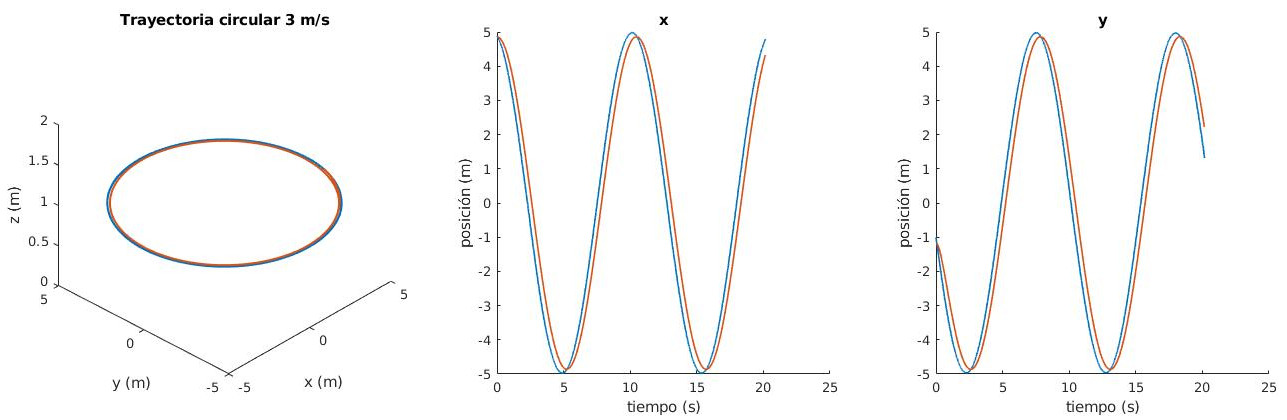
\includegraphics[width=\textwidth]{imagenes/circle3ms}
	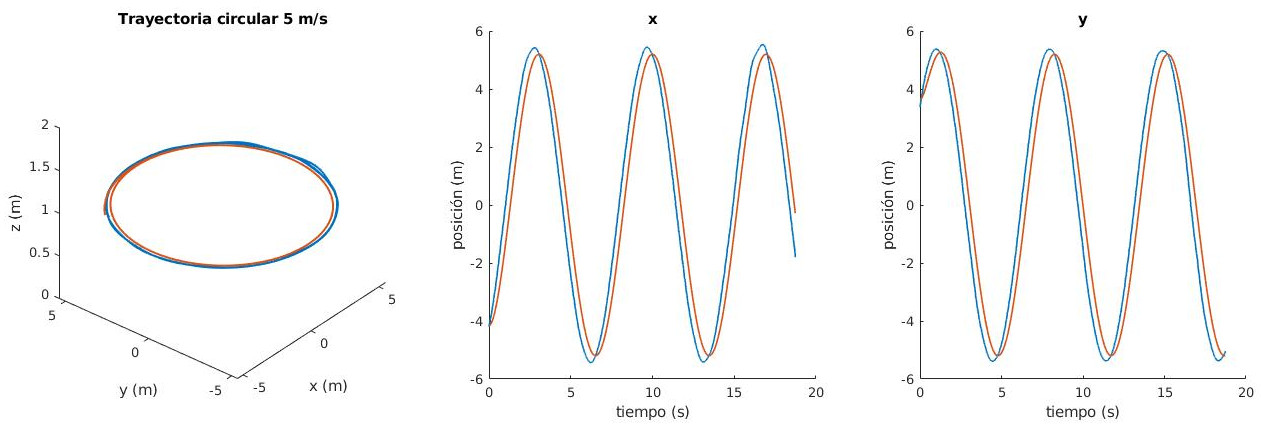
\includegraphics[width=\textwidth]{imagenes/circle5ms}
	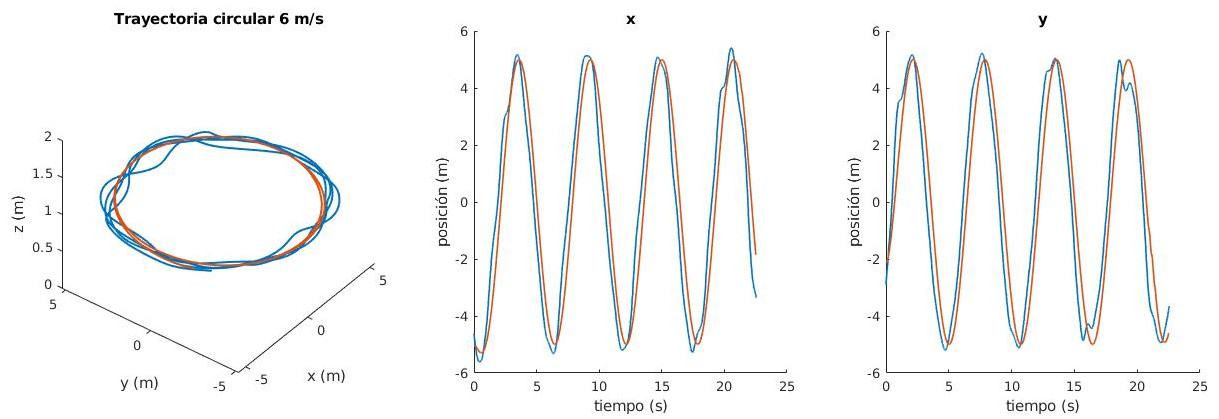
\includegraphics[width=\textwidth]{imagenes/circle6ms}
	\caption{Trayectorias circulares a 3, 5 y 6 m/s empleando un controlador para ángulos pequeños. La trayectoria a seguir se muestra en rojo, mientras que la trayectoria seguida por el cuadricóptero se muestra en azul.}	\label{circle:slow}
\end{figure}
\newpage
\subsection{Controlador grandes  ángulos}

\begin{figure}[htb!]
	\centering
	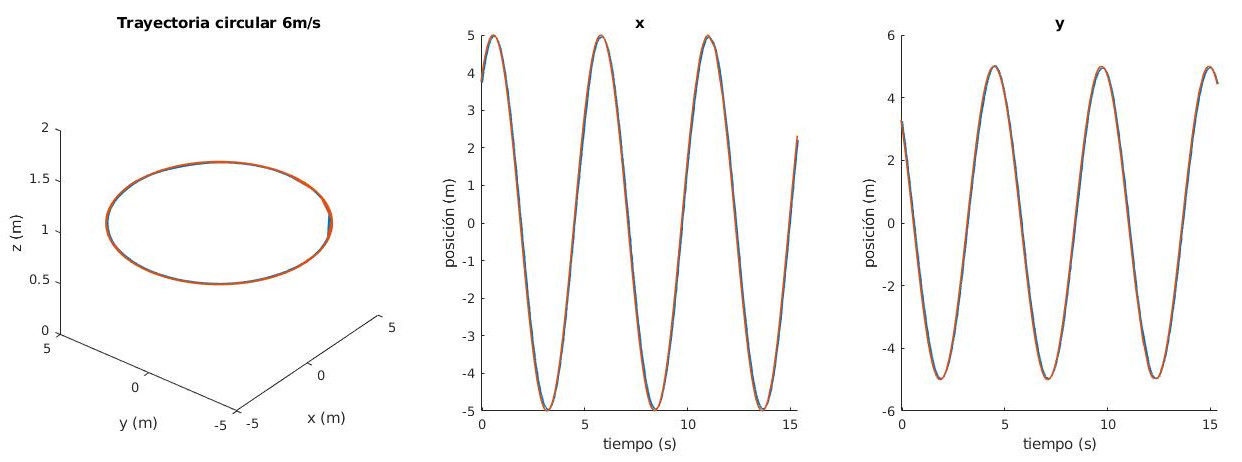
\includegraphics[width=\textwidth]{imagenes/fast_circle6ms}
	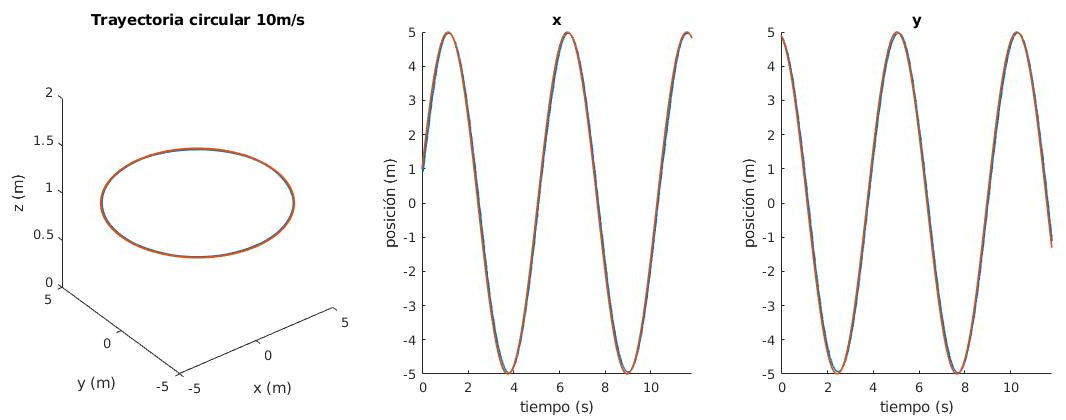
\includegraphics[width=\textwidth]{imagenes/fast_circle10ms}
	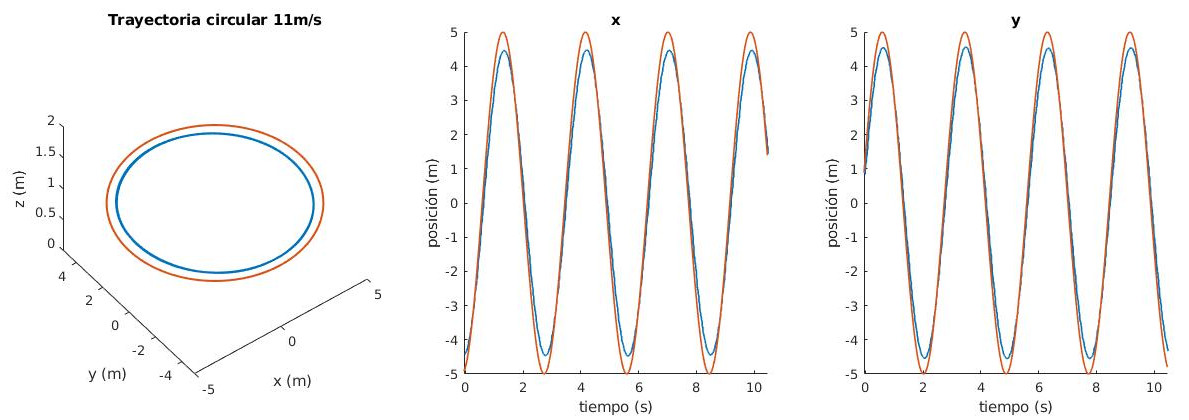
\includegraphics[width=\textwidth]{imagenes/fast_circle11ms}
	\caption{Trayectorias circulares a 6, 10 y 11 m/s empleando un controlador para ángulos grandes. La trayectoria a seguir se muestra en rojo, mientras que la trayectoria seguida por el cuadricóptero se muestra en azul.}
	\label{circle:fast}
\end{figure}
\newpage

\section{Recorrido del circuito de carreras}

Para realizar los experimentos del recorrido completo del circuito se han empleado las mismas condiciones impuestas en las pruebas clasificatorias del AlphaPilot 2019. En estas pruebas las posiciones aproximadas de las puertas son conocidas a priori por el sistema, así como los indicadores de cada puerta vista por las cámaras y las posiciones de las esquinas de las mismas en la imagen como se supuso en el apartado \ref{section:gen_traj}.
En la arquitectura completa se ha optado por emplear el controlador para grande ángulos debido a que consigue alcanzar velocidades más altas de forma robusta. 

Se ha recorrido el circuito con dos configuraciones distintas de las limitaciones dinámicas del sistema en la generación de trayectorias a corto plazo: Una configuración con valores más conservadores de velocidad y acceleración máximas y otra configuración con valores maś extremos de velocidad y aceleración máximas . A continuación se muestran los resultados obtenidos con cada configuración y las gráficas obtenidas durante el recorrido del circuito. Las trayectorias generadas mostradas en los gráficos corresponden a las referencias de posición obtenidas por el controlador a lo largo de todo recorrido, por lo que corresponden al muestreo de la trayectoria a corto plazo a lo largo del circuito.

\subsection{Configuración de velocidad conservadora.}

Los parámetros empleados durante la generación de trayectorias en este experimento son $A_{max} = 2g $ $(m/s^2)$ y $V_{max} = 8$ $(m/s)$. El tiempo necesario para completar el circuito completo fue de 32.93 $s$.
\vspace{2cm}
\begin{figure}[htb!]
	\centering
	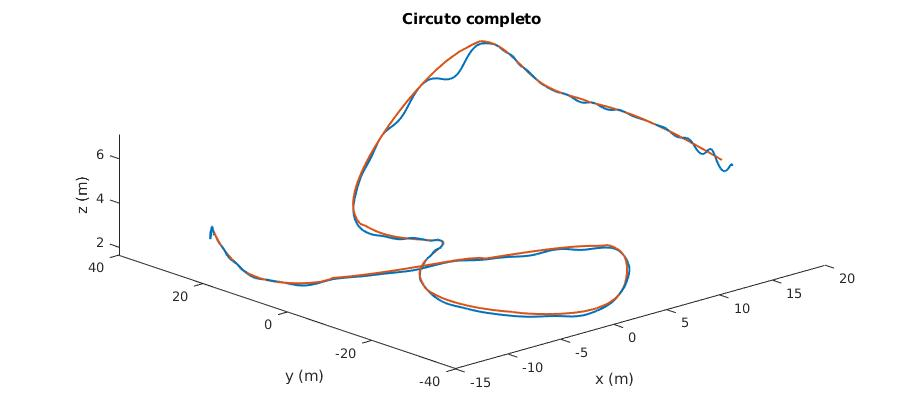
\includegraphics[width=\textwidth]{imagenes/circuitFigure}
	\caption{Trayectoria 3D planificada a lo largo del circuito (roja) y el recorrido realizado por el cuadricóptero (azul).}
	\label{exp1:1}
\end{figure}

\begin{figure}[htb!]
	\centering
	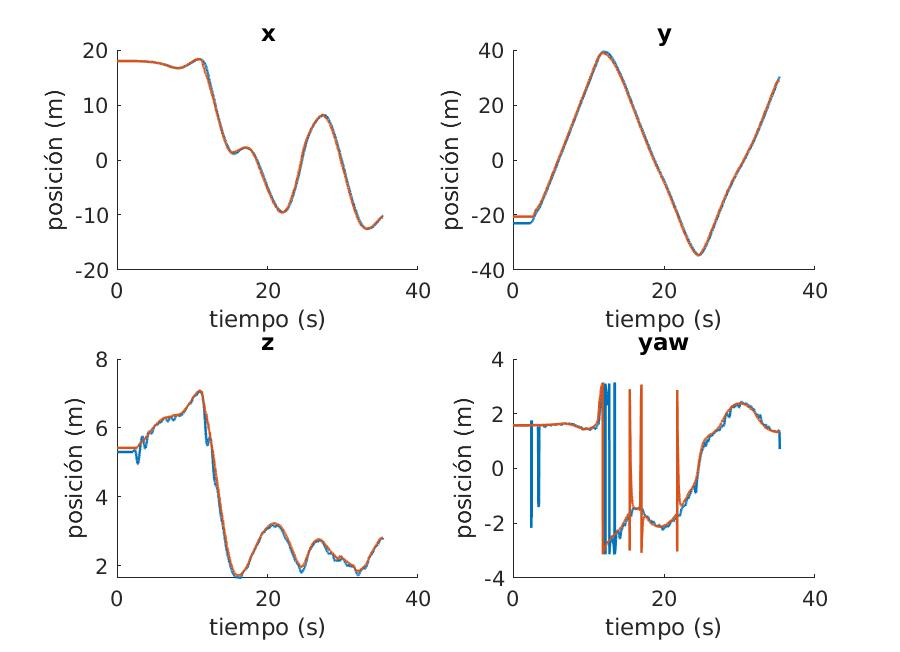
\includegraphics[width=0.85\textwidth]{imagenes/positionFigure}
	\caption{Trayectoria por coordenadas  planificada a lo largo del circuito (roja) y el recorrido realizado por el cuadricóptero (azul).}
	\label{exp1:2}
\end{figure}

\begin{figure}[htb!]
	\centering
	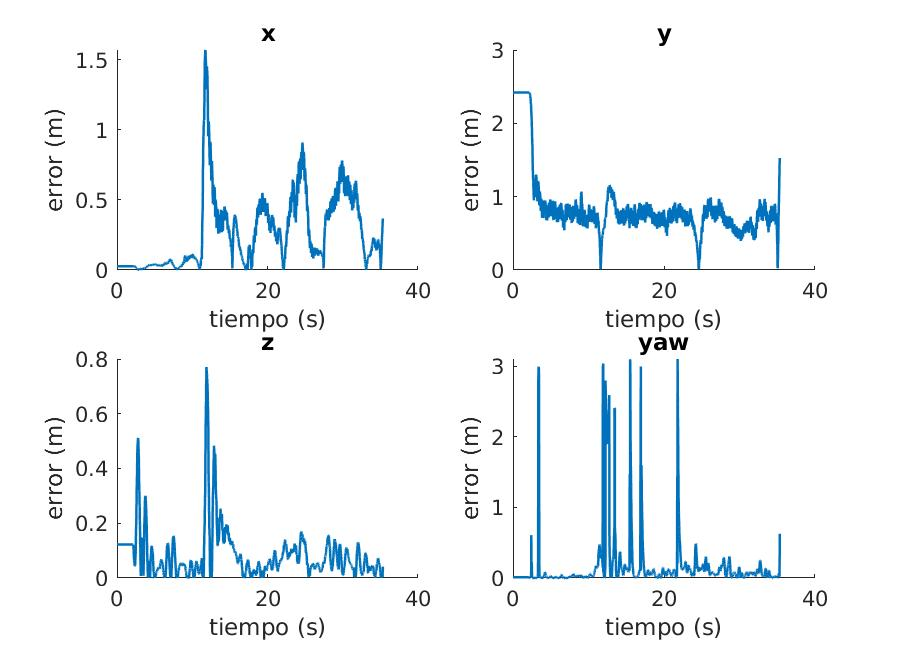
\includegraphics[width=0.90\textwidth]{imagenes/errorFigure}
	\caption{Errores de seguimiento entre la trayectoria planificada y la trayectoria seguida coordenada por coordenada.}
	\label{exp1:3}
\end{figure}
\newpage
De las gráficas obtenidas anteriormente se pueden obtener el valor medio y máximo de los errores de seguimiento en cada eje, así como las velocidades medias y máximas obtenidas durante el recorrido.


\begin{table}[htb!]
	\centering
	\begin{tabular}{l|c|c|c|}
		$\empty$&Eje x&Eje y&Eje z\\
		\midrule
		Error máximo (m)&1.5685&1.1577&0.7707\\
		Error medio (m) &0.3143&0.7306&0.0796\\
	\end{tabular}
	\caption{Errores de seguimiento durante el recorrido del circuito.}
		\label{table_error_1}
\end{table}


\begin{table}[htb!]
	\centering
	\begin{tabular}{l|c|c|}
		$\empty$&Máxima& Media\\
		\midrule
		Velocidad (m/s)&7.4119&5.7248\\
	\end{tabular}
	\caption{Velocidad del cuadricóptero durante el recorrido del circuito.}
	\label{table_speed_1}
\end{table}

\subsection{Configuración de máxima velocidad.}

Los parámetros empleados durante la generación de trayectorias en este experimento son $A_{max} = 4g $ $(m/s^2)$ y $V_{max} = 12$ $(m/s)$. El tiempo necesario para completar el circuito completo fue de 22.34 $s$.
\vspace{1.6cm}

\begin{figure}[htb!]
	\centering
	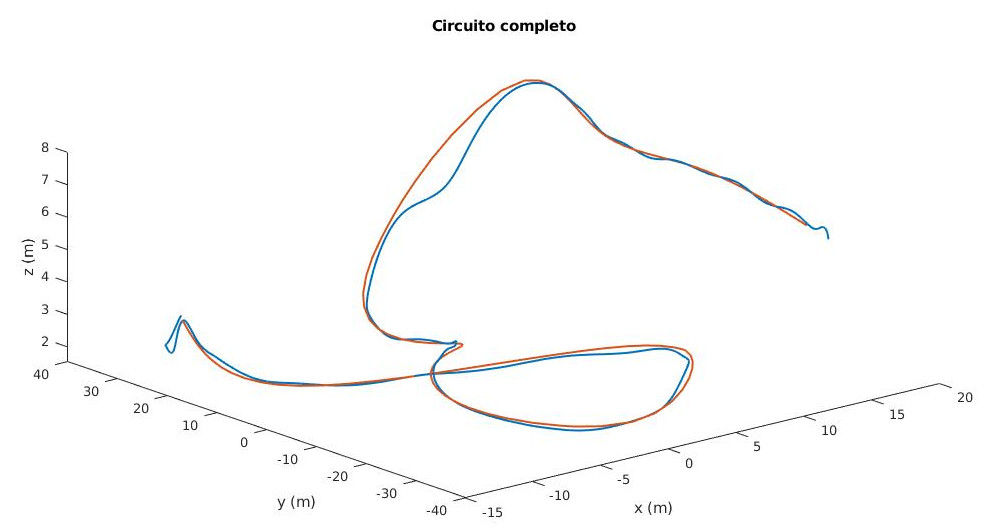
\includegraphics[width=\textwidth]{imagenes/best_circuitFigure}
	\caption{Trayectoria 3D planificada a lo largo del circuito (roja) y el recorrido realizado por el cuadricóptero (azul).}
	\label{exp:1}
\end{figure}
\newpage
\begin{figure}[htb!]
	\centering
	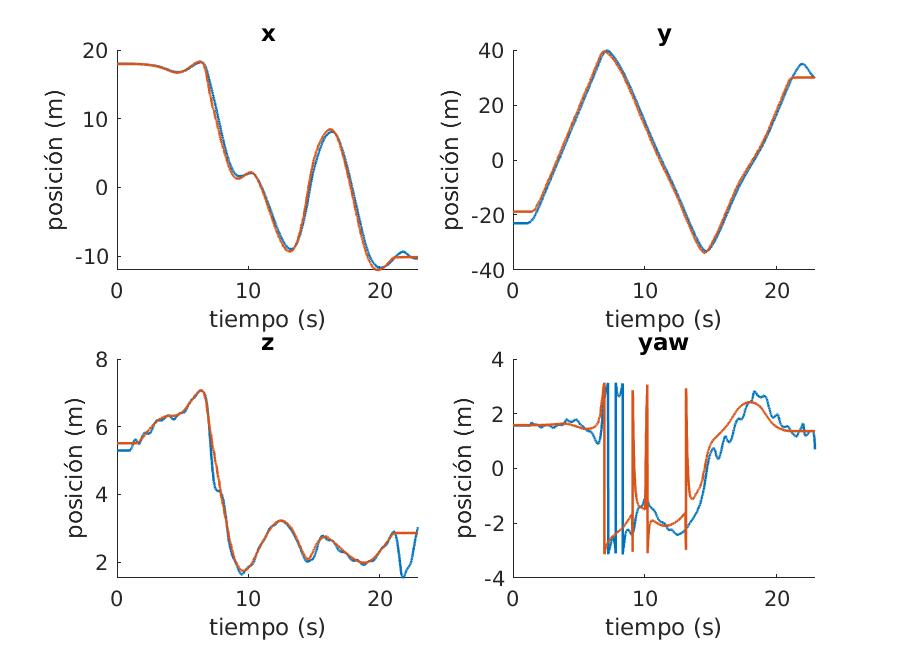
\includegraphics[width=0.85\textwidth]{imagenes/best_positionFigure}
	\caption{Trayectoria por coordenadas  planificada a lo largo del circuito (roja) y el recorrido realizado por el cuadricóptero (azul).}
	\label{exp2:2}
\end{figure}

\begin{figure}[htb!]
	\centering
	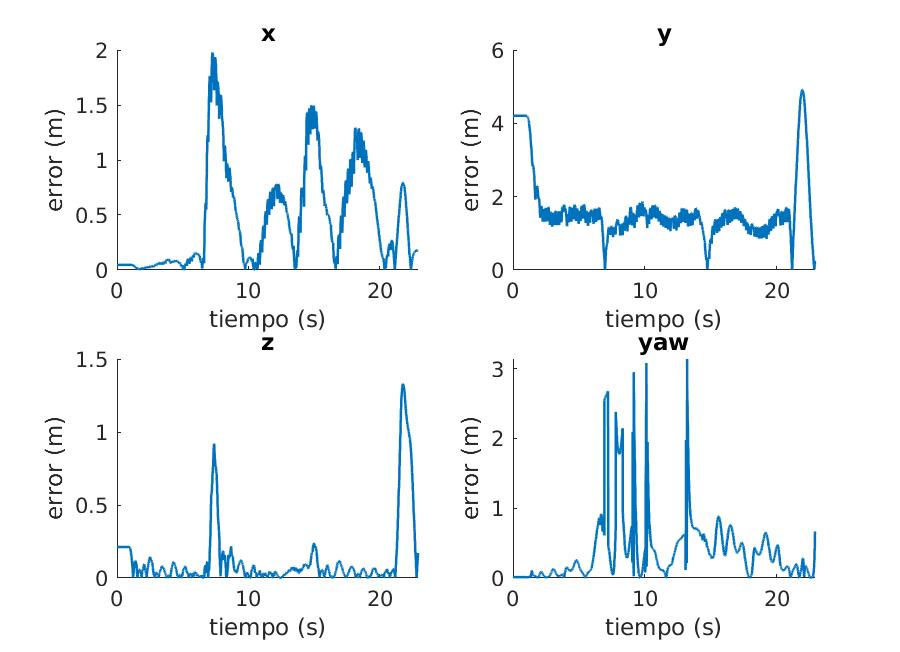
\includegraphics[width=0.85\textwidth]{imagenes/best_errorFigure}
	\caption{Errores de seguimiento entre la trayectoria planificada y la trayectoria seguida coordenada por coordenada.}
	\label{exp2:3}
\end{figure}

\newpage
De las gráficas obtenidas anteriormente se pueden obtener el valor medio y máximo de los errores de seguimiento en cada eje, así como las velocidades medias y máximas obtenidas durante el recorrido.

\begin{table}[htb!]
	\centering
	\begin{tabular}{l|c|c|c|}
		$\empty$&Eje x&Eje y&Eje z\\
		\midrule
		Error máximo (m)&1.9776&1.9181&1.3302\\
		Error medio (m) &0.5973&1.4826&1.1413\\
		
	\end{tabular}
	\caption{Errores de seguimiento durante el recorrido del circuito.}
	\label{table:error:2}
\end{table}



\begin{table}[htb!]
	\centering
	\begin{tabular}{l|c|c|}
		$\empty$&Máxima& Media\\
		\midrule
		Velocidad (m/s)&10.4948&9.3936\\
		
	\end{tabular}
	\caption{Velocidad del cuadricóptero durante el recorrido del circuito.}
	\label{table:speed:2}
\end{table}

\chapter{Discusión de resultados.}

A continuación se discutirán los resultados obtenidos en el capítulo anterior.

\section{Comparación entre controladores}

En las figuras \ref{circle:slow} y \ref{circle:fast} se puede observar como ambos controladores son capaces de seguir la trayectoria propuesta correctamente a bajas velocidades. Sin embargo, se puede observar como el error de seguimiento del controlador para ángulos pequeños aumenta a medida que se incrementa la velocidad, comenzando a perder la estabilidad al alcanzar velocidades de unos 6 m/s. Debido al tamaño de la circunferencia escogido, cuando el cuadricóptero se aproxima a estas velocidades los ángulos de roll $\phi $ y pitch $\theta$ comienzan a crecer, por lo que la linealización en torno al estado de hover comienza a fallar, provocando las oscilaciones que se pueden observar en la 3ª gráfica de la figura \ref{circle:slow}.

El controlador para grandes ángulos es capaz de sobrepasar esta velocidad sin problemas, llegando a velocidades de unos 10 m/s manteniendo un bajo error de seguimiento, como se puede observar en la figura \ref{circle:fast}. A partir de esta velocidad, se observa como el cuadricóptero comienza a alejarse de la trayectoria propuesta. Este fenómeno se puede deber a que se alcanza el empuje máximo que pueden dar los motores del aeronave, lo que satura la señal de control del aeronave, provocando que se llegue a una situación de equilibrio con un cierto error de seguimiento. 

Con este análisis cualitativo se manifiestan los comportamientos esperados por ambos controladores: el controlador para ángulos pequeños se comporta bien a bajas velocidades, empeorando su rendimiento a medida que aumenta la inclinación del aeronave, mientras que el controlador para grandes ángulos es capaz de volar a velocidades más elevadas de una forma más robusta. Es por esto que se decide emplear el controlador para grandes ángulos durante los experimentos del recorrido del circuito de carreras.

\section{Recorrido del circuito de carreras}

En los dos experimentos realizados con distintas configuraciones, se consigue recorrer el circuito entero de forma satisfactoria, atravesando las 11 puertas del circuito en el orden indicado sin colisionar con el entorno. Comparando las tablas \ref{table_speed_1} y \ref{table:speed:2}, se observa que con la configuración más agresiva se consigue aumentar de forma considerable la velocidad media a la que el aeronave recorre el circuito, obteniendo un aumento de un 60\% respecto a la configuración más conservadora. Sin embargo, en las figuras \ref{exp1:3} y \ref{exp2:3}  y en las tablas \ref{table_error_1} y \ref{table:error:2} se observa como el error de seguimiento también aumenta de forma considerable en la configuración más agresiva, llegando a duplicar el error medio en cada eje. Este aumento hace que sea más arriesgado usar está configuración ya que se aumenta considerablemente el riesgo de colisión al atravesar una puerta, además las velocidades de vuelo más elevadas también empeoran la calidad de las estimaciones del módulo de percepción, lo que aumenta aún más el riesgo de colisión. Los errores de seguimiento más elevados se encuentran entre los cambios en las trayectorias a corto plazo, debido a la discontinuidad existente entre las referencias enviadas al controlador.

En ambos casos los módulos de generación de trayectorias son capaces de generar trayectorias a corto y largo plazo adecuadas y de actualizarlas a altas frecuencias con las nuevas mediciones obtenidas por el módulo de percepción, consiguiendo que el aeronave sea capaz de recorrer el circuito de forma satisfactoria a velocidades muy elevadas.
Asimismo, el cuadricóptero tardo menos de 35 segundos en completar el circuito en ambos casos, lo que estaría dentro de los tiempos que consiguieron los 3 mejores obtenidos en las pruebas clasificatorias del AlphaPilot 2019 \cite{guerra2019flightgoggles}. Sin embargo, a diferencia de las pruebas de la competición, en este trabajo se ha empleado la estimación de estado provista por el simulador, mientras que en las pruebas oficiales el módulo de percepción también debe ser implementado. 





